\section{Módulo de Calendario y Actividades}

El módulo de \textbf{Calendario} en Odoo es la herramienta central para organizar el tiempo de tu equipo. Está sincronizado con todo el sistema, lo que significa que cualquier actividad programada desde el CRM (como llamar a un pasajero) o desde Ventas aparecerá automáticamente aquí.

\subsection{1. Vista General del Calendario}

Al ingresar al módulo, verás una cuadrícula tradicional. En el panel izquierdo tienes un pequeño calendario mensual y una lista de los calendarios de otros miembros del equipo (que puedes marcar o desmarcar para ver en qué andan tus compañeros).

\begin{figure}[H]
    \centering
    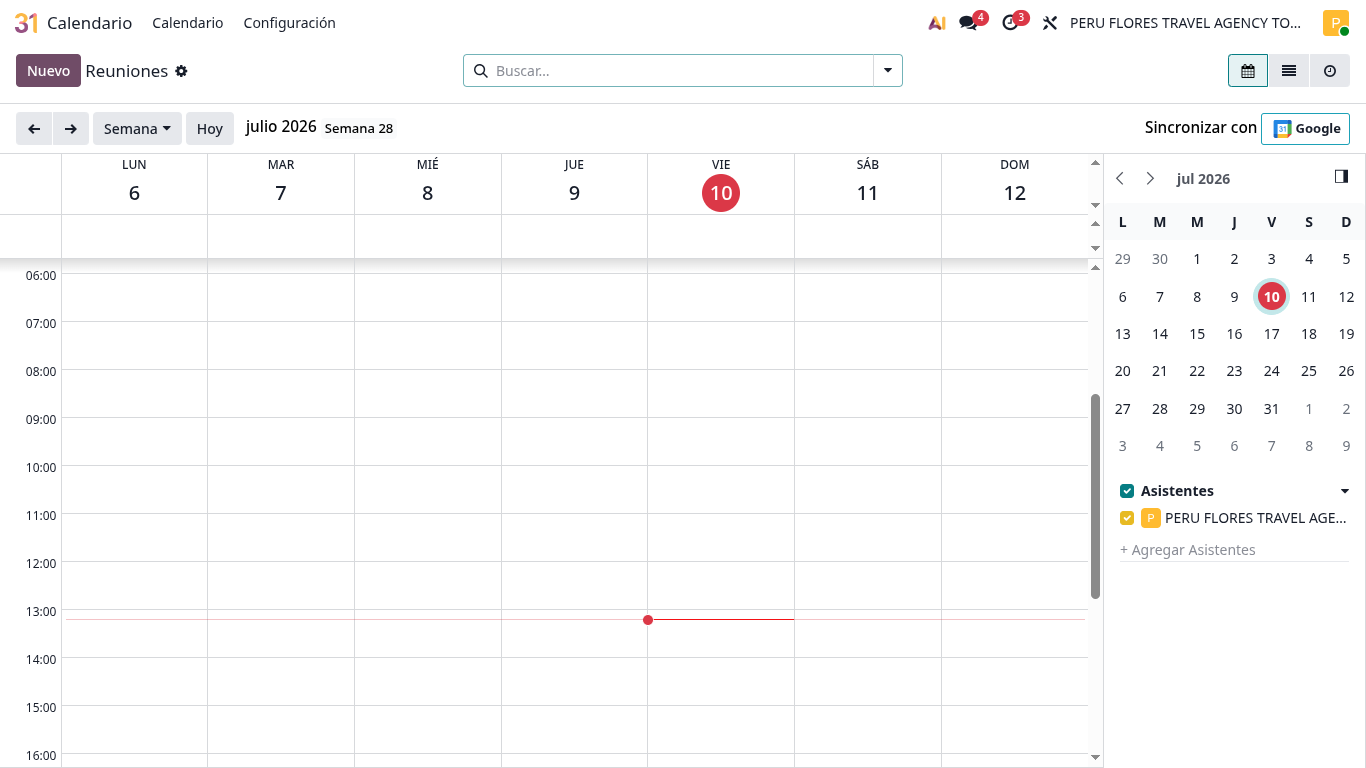
\includegraphics[width=0.9\textwidth]{assets/cal_01_vista_mensual.png}
    \caption{Vista principal del calendario. Puedes cambiar entre vista de Día, Semana, Mes o Año en la parte superior derecha.}
\end{figure}

\subsection{2. Agendar una cita (Modo Rápido)}

Para agendar una actividad rápidamente (una reunión de equipo, un recordatorio de cobro, etc.):
\begin{itemize}
    \item Haz clic en cualquier recuadro vacío del calendario que corresponda al día u hora deseada.
    \item Aparecerá un cuadro flotante donde solo necesitas colocar el \textbf{Asunto} de la reunión.
    \item Al presionar \textbf{``Crear''}, el evento quedará agendado instantáneamente.
\end{itemize}

\begin{figure}[H]
    \centering
    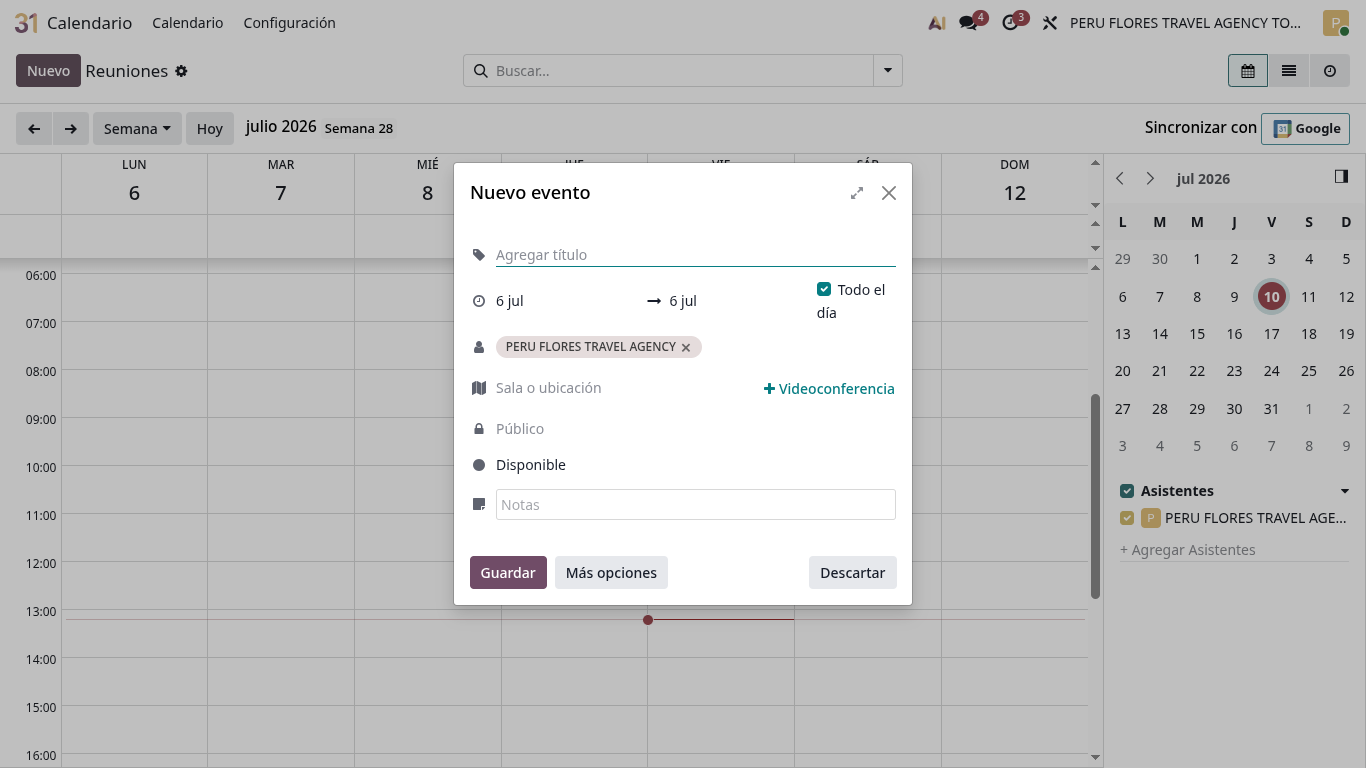
\includegraphics[width=0.9\textwidth]{assets/cal_02_crear_cita.png}
    \caption{Ventana flotante de creación rápida de citas al hacer clic en un día del calendario.}
\end{figure}

\subsection{3. Agendar una cita (Formulario Completo)}

Si tu reunión requiere más detalles, como invitar a otras personas para que les llegue un correo de notificación, configurar videollamadas o agregar una descripción larga:

\begin{itemize}
    \item En lugar de darle a ``Crear'' en el cuadro flotante, haz clic en el botón \textbf{``Editar''} o \textbf{``Más opciones''}.
    \item Se abrirá el formulario completo del evento.
\end{itemize}

\begin{figure}[H]
    \centering
    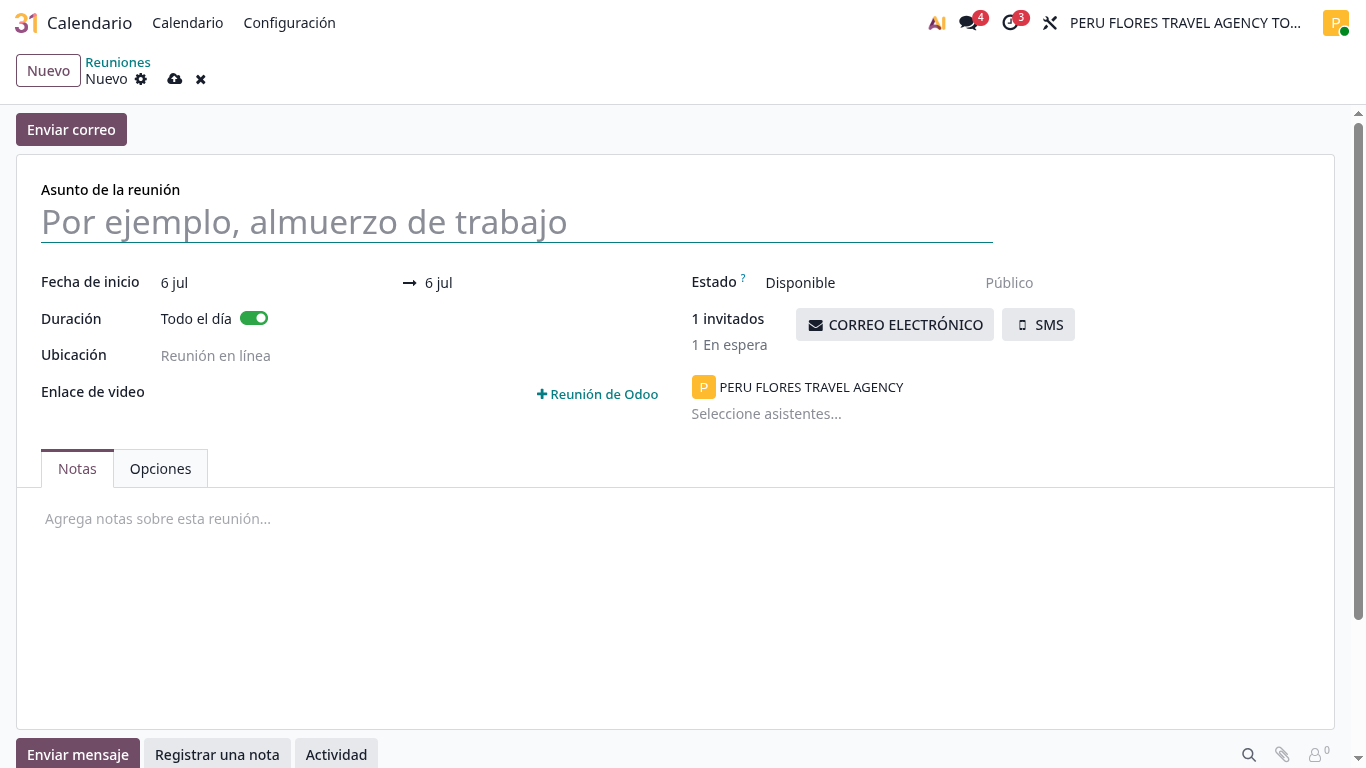
\includegraphics[width=0.9\textwidth]{assets/cal_03_formulario_completo.png}
    \caption{Formulario detallado de un evento del calendario.}
\end{figure}

Al entrar al formulario, debes llenar estos campos principales:
\begin{itemize}
    \item \textbf{Asunto (Título):} El motivo principal de la reunión (Ej: "Llamada de ventas - Pasajero Carlos").
    \item \textbf{Asistentes:} Escribe los nombres o correos de las personas que deben participar. Al guardarlo, Odoo les enviará automáticamente un correo de invitación con archivo adjunto (.ics) para que lo agreguen a su calendario de Google o Outlook.
    \item \textbf{Videollamada:} Si vas a tener una reunión virtual, Odoo puede generar un \textbf{enlace de reunión de Odoo} nativo para no depender de Zoom u otros.
    \item \textbf{Ubicación:} Para reuniones físicas o para dejar el enlace de Google Meet/Zoom si prefieres usar un servicio externo.
    \item \textbf{Etiquetas:} Selecciona la clasificación (ej: Interno, Cliente, Proveedor) para que el evento adquiera un color específico en el calendario general y sea fácil de distinguir.
    \item \textbf{Recordatorios:} Configura notificaciones para que el sistema te avise 15 minutos, 1 hora o 1 día antes por la campanita del sistema o por correo electrónico.
    \item \textbf{Descripción:} Usa el cuadro de texto inferior para apuntar la agenda de la reunión o notas para los asistentes.
\end{itemize}

\subsection{4. Ver, Editar y Eliminar Eventos (Gestión y CRUD)}

Una vez que un evento ha sido creado y aparece en el calendario, puedes gestionarlo de la siguiente manera:

\begin{itemize}
    \item \textbf{Ver detalles (Read):} Haz clic simple sobre cualquier recuadro de color en el calendario. Se abrirá una pequeña ventana (pop-over) con el resumen de la reunión y los enlaces rápidos.
    \item \textbf{Editar (Update):} Dentro de esa pequeña ventana, encontrarás el botón \textbf{``Editar''} (marcado en la siguiente figura). Esto te devolverá al formulario completo para modificar asistentes o la fecha. También puedes simplemente \textbf{arrastrar y soltar (Drag and Drop)} el evento de un día a otro directamente en la cuadrícula.
    \item \textbf{Eliminar (Delete):} Si la reunión se canceló por completo y deseas borrar el registro, usa el botón \textbf{``Eliminar''} que aparece en rojo en la misma ventanita.
\end{itemize}
